\documentclass[14pt]
{article}

%basiques
\usepackage[utf8x]{inputenc}
\usepackage[T1]{fontenc}
\usepackage[english]{babel}

%math
\usepackage{amsmath}
\usepackage{amssymb}

% images
\usepackage{graphicx, float}
\usepackage{subcaption}

%mise en page
\usepackage{fancyhdr}
\usepackage{fancybox}
\usepackage[margin=3cm]{geometry}
\usepackage[colorlinks]{hyperref}
\usepackage[nameinlink,noabbrev]{cleveref}

\newcommand\tab[1][1cm]{\hspace*{#1}}

%\geometry{hmargin=3cm}

\begin{document}
% Entete
\pagestyle{fancy}
\lhead{Léa Heiniger}
\rhead{31.10.2022}
\chead{\textbf{Metaheuristics for optimization}}

\bigskip
\begin{center}
	\section*{\textbf{{\LARGE TP3 : Simulated Annealing and Parallel Tempering for the Traveling Salesman Problem}}}
\end{center}
\bigskip\bigskip\bigskip

%%%%%%%%%%%%%%%%%%%%%%%%%%%%%%%%%% Introduction %%%%%%%%%%%%%%%%%%%%%%%%%%%%%%%%%%
\section{Introduction}
In this TP we are working on the Travelling Salesman Problem (TSP). In this problem we have a set of $N$ cities and the coordinates of their locations and we want to find the shortest path such that every city is visited exactly one time.

\subsection{Simulated Annealing}
To resolve this problem the metaheuristics we will be using is the Simulated Annealing (SA). This algorithm was designed to copy the natural effect of annealing (when a metal heated cools down progressively). The goal is to find a state with a minimal energy. The principle is to start wit a high initial temperature that represents the probability of accepting worse solutions and as we iterate we will reduce the temperature (meaning we increase the probability of accepting better solutions) until we reach a frozen point.\\
To apply it to the TSP each state will represent a possible path (going through all cities exactly once) and its energy will be the total length of that path. A path is a loop so when we compute the energy of a path we must include the distance between the last city and the first one.
%%%%%%%%%%%%%%%%%%%%%%%%%%%%%%%%%% Implementation %%%%%%%%%%%%%%%%%%%%%%%%%%%%%%%%%%
\section{Implementation}
The implementation of this problem can be found in the files \texttt{TP3.py} and \texttt{functions.py}.The file \texttt{functions.py} is a library of functions created for this TP and \texttt{TP3.py} contains the code that allows us to compute the algorithms several times and to display the results.\\
\\
To run the code we simply need to run the following command in a Terminal :\\
\texttt{python3 TP3.py <data file name>}\\
Where \texttt{<data file name>} is an optional argument, if we want to run the code on a task described in a data file we replace it by the file name otherwise the code will be run on randomly generated tasks.\\
\\
The file \texttt{circle.dat} is the file describing cities placed around a circle and was used to test the implementation.

\subsection{The Travelling Salesman Problem}
The states of a TSP are represented as a list of cities. Each city is a list of the form $[name, x ,y]$ where $name$ is the name of the city and $x$ and $y$ are the coordinates of the city.\\
\\
Representation of a state from the TSP described in file \texttt{cities.dat} :\\
\texttt{[['a', 0.0, 0.0], ['b', 0.0, 1.0], ['c', 1.0, 0.0], ['d', 2.0, 2.0], ['e', 0.5, 3.0], ['f', 3.0, 0.5], ['g', 4.0, 4.0], ['h', 3.0, 0.0], ['i', 4.0, 1.0], ['j', 1.3, 2.0], ['k', 1.0, 6.0], ['l', 2.0, 3.0], ['m', 7.5, 3.0], ['n', 0.5, 1.3], ['o', 2.0, 6.0], ['p', 6.0, 3.0], ['q', 3.0, 2.0], ['r', 0.0, 6.0]]}\\
\\
In the file \texttt{functions.py} there are two functions. The first one, \texttt{extract\_cities} that extract the data from a task file and returns it as a list of cities, and the second one, \texttt{random\_TSP}, that creates a random TSP with $N$ cities.

\begin{figure}[h] %%%%%%%%%%%%%%%%%%%%%%%%%%%%%%%%%%%%%%%%%%%%%%%%%%
\center
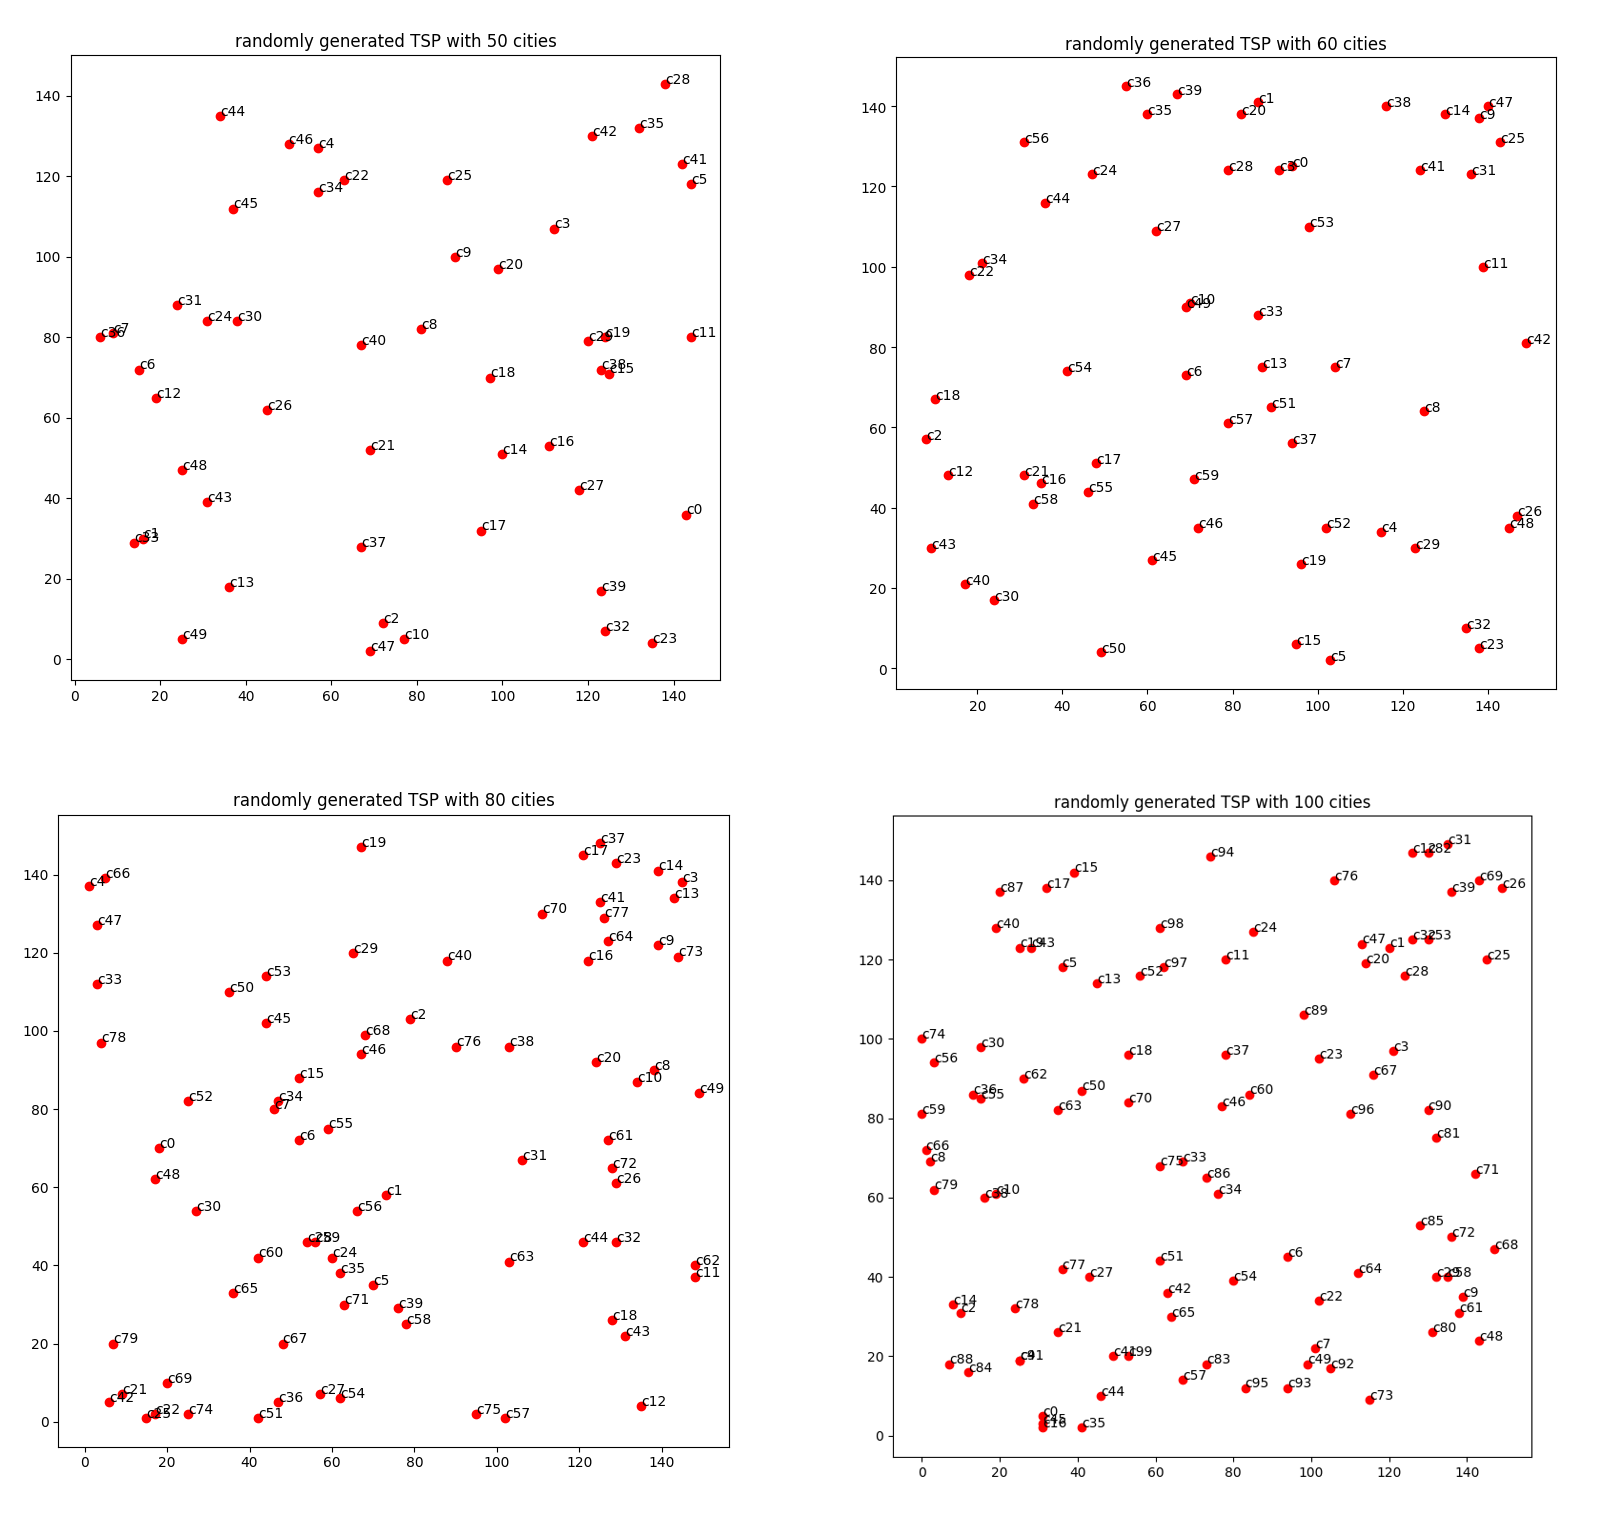
\includegraphics[scale=1]{img/randTSP.png}
\caption{Examples of randomly generated TSP}
\end{figure}

\subsection{Greedy Algorithm}
Since we want to compare the results of the simulated annealing to the results of the greedy algorithm I needed to implement it as well. For the TSP the greedy algorithm consist in taking the closest city at each steps. In order to achieve that I created two functions, \texttt{distance} that compute the distance between two cities and \texttt{closest} that returns the closest city from a given city. Those two functions are used in the function \texttt{greedy} that implements the greedy algorithm for the TSP.

\subsection{Simulated Annealing}
The simulated annealing algorithm for the TSP is implemented in the function \texttt{simulate\_annealing}. For this implementation I followed the phases describes in the TP instructions and for some of them other functions were needed :
\begin{itemize}
\item For the \textbf{initial configuration} I created a function \texttt{random\_path} that generates a random initial path keeping the first city as the start.

\item To compute the \textbf{initial temperature} I created a function \texttt{init\_temperature} that is based on the equation $e^{\frac{-\left\langle \vert \Delta E\vert\right\rangle}{T_{0}}} = 0.5$. This function calls three other functions, that are also useful for the \textbf{elementary configuration update}, \texttt{permutations} that returns a list of possible permutations of two cities from a given state, \texttt{transition} that perform a permutation of two cities and \texttt{energy} that compute the energy (length) of a path.

\item Finally I created two functions returning a boolean, one named \texttt{equilibrium} that check if the \textbf{equilibrium conditions} are fulfilled and the other named \texttt{frozen} that does the same for the \textbf{freezing conditions}.

\end{itemize}

%%%%%%%%%%%%%%%%%%%%%%%%%%%%%%%%%% Results %%%%%%%%%%%%%%%%%%%%%%%%%%%%%%%%%%
\section{Results}

\subsection{Tasks from a file}
First I will focus on the results obtained on the two tasks provided in files \texttt{cities.dat} and \texttt{cities2.dat}. As suggested I started by testing my implementation on a TSP with all cities put on a circle. We can see on \autoref{circle} that both algorithms have found the optimal solution (with an energy of $61.91015106167883$) as we expected it.

\begin{figure}[H] 
\center
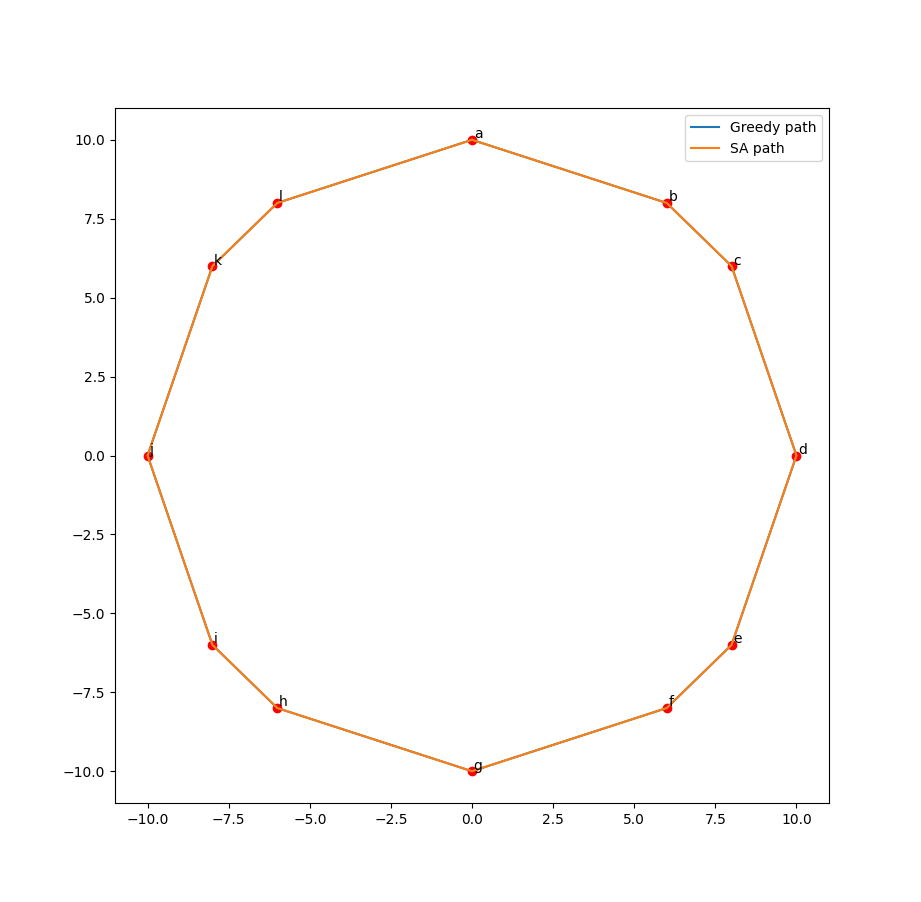
\includegraphics[scale=0.3]{img/circle.png}
\caption{\label{circle} Example of Greedy and SA solutions for a TSP with cities put on a circle}
\end{figure}

\subsubsection{\texttt{cities.dat}}

\begin{figure}[H]
\center
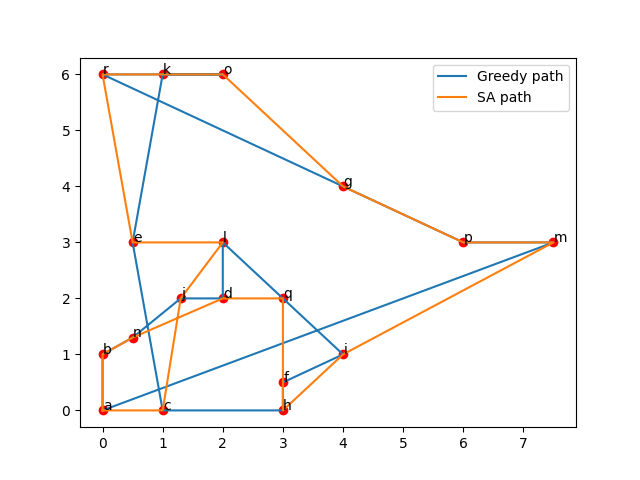
\includegraphics[scale=0.5]{img/cities.png}
\caption{Example of Greedy and SA solutions for file \texttt{cities.dat}}
\end{figure}

As we can see on \autoref{cities} the energy of the solutions found by the greedy algorithm is always $36.16128455775342$. This is expected since the algorithm will always make the same choice (the closest city) at each steps and will return the same solution each time. With the simulated annealing we have a lot of different solutions. Again this is expected since it is a probabilistic algorithm. The best energy fond is  $29.032638932315717$ which is much better than the one found with the greedy algorithm. We can see that the mean of the values found $32.717604344196495$ is a bit higher but still better than the on found with the greedy algorithm. But the higher energy found is $36.57932973855604$ which is worse than the solution found with the greedy algorithm. 

\begin{figure}[H]
\center
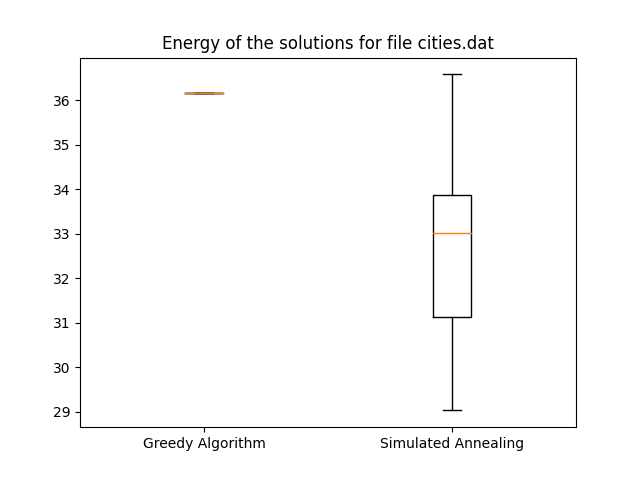
\includegraphics[scale=0.5]{img/box_cities.png}
\caption{\label{cities} Box-plot for the file \texttt{cities.dat}}
\end{figure}

\subsubsection{\texttt{cities2.dat}}

\begin{figure}[H] 
\center
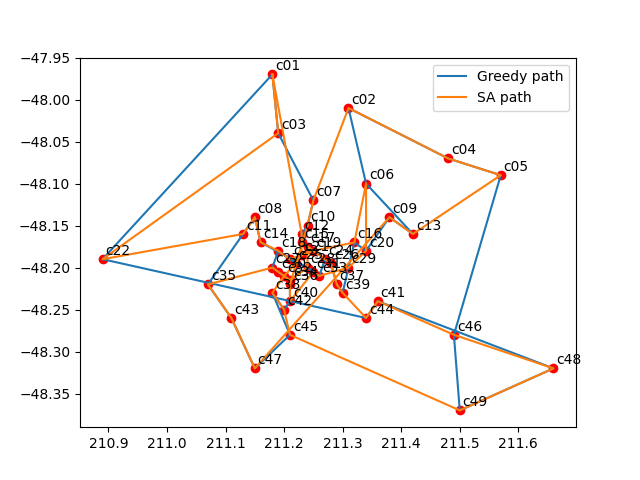
\includegraphics[scale=0.5]{img/cities2.png}
\caption{Example of Greedy and SA solutions for file \texttt{cities2.dat}}
\end{figure}

On \autoref{cities2} we can see that as previously the greedy algorithm always finds the same solution with an energy of $3.303495043530876$. The best solution found by the simulated annealing algorithm is better with an energy of $3.245685674879906$ but this time the mean of the energies found is $3.598667748909031$ which is higher than the energy from the greedy solution.
\newpage

\begin{figure}[H] 
\center
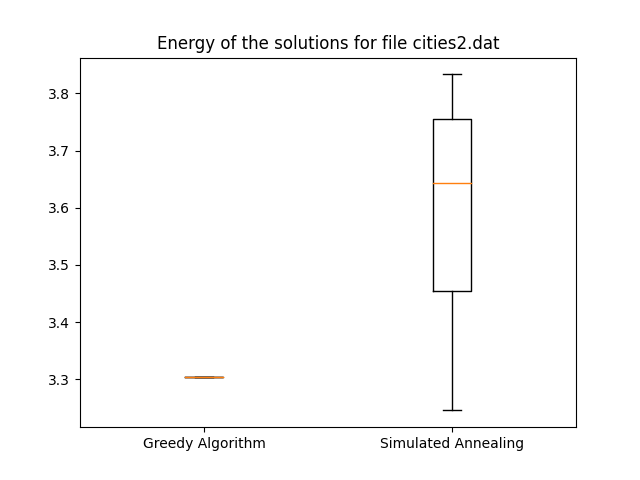
\includegraphics[scale=0.5]{img/box_cities2.png}
\caption{\label{cities2} Box-plot for the file \texttt{cities2.dat}}
\end{figure}

From the results on those two tasks we can conclude that that simulated annealing can find better solutions than the greedy algorithm (when the greedy solution is not the optimal solution otherwise we can't do better). But it doesn't always find a better solution and when run several times most of the values are higher than the energy of the best solution. We could improve this by using the 2-opt permutation method.

\subsection{Randomly generated tasks}
In this section I will look at the results obtained on randomly generated TSP. For each number of cities $N$ I generated a TSP randomly using the function \texttt{random\_TSP} and ran 10 times both algorithms on it. 

\subsubsection{Energy}
On \autoref{EBoth} we can see that as before the greedy algorithm always finds the same solution. But this time the simulated annealing finds worse solutions each time. Even the best energy found with the SA algorithm is far worse than the greedy.\\
The gap size between the greedy solution and the SA solution depends of the TSP generated. For some of them (with the same $N$) the best energy found by the simulated annealing was closer to the energy found with the greedy algorithm, but always higher.\\

\begin{figure}[H]
\centering
\begin{subfigure}{0.49\textwidth}
\centering
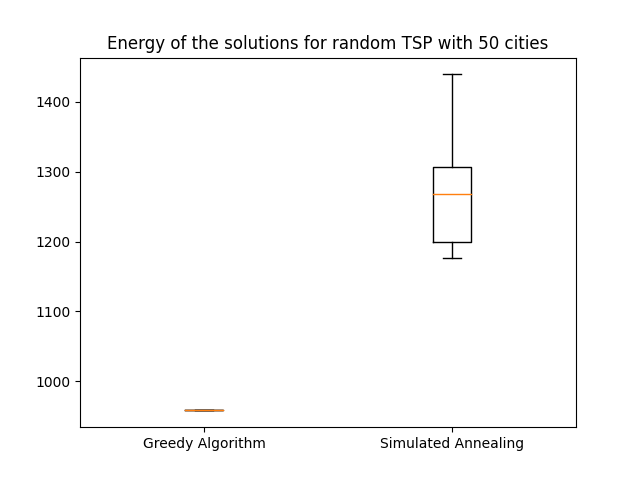
\includegraphics[width = \textwidth]{img/E50.png}
\end{subfigure}
\begin{subfigure}{0.49\textwidth}
\centering
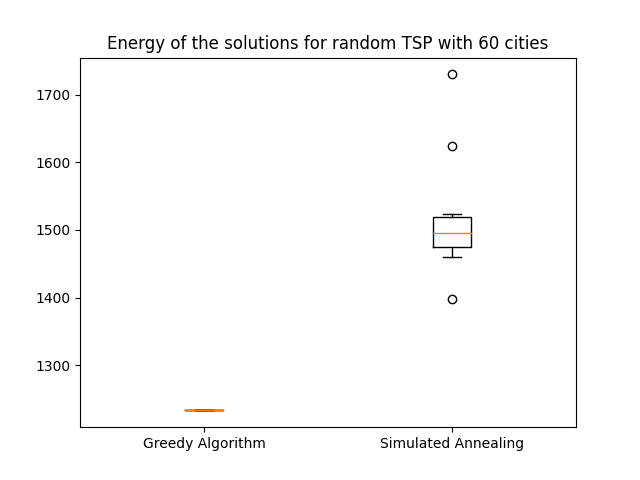
\includegraphics[width = \textwidth]{img/E60.png}
\end{subfigure}
\begin{subfigure}{0.49\textwidth}
\centering
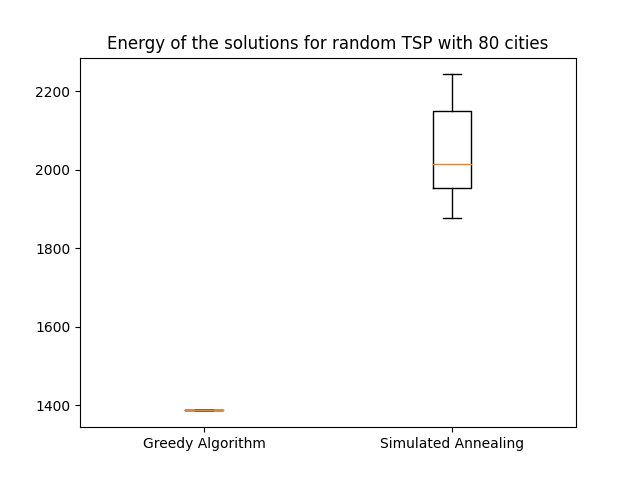
\includegraphics[width = \textwidth]{img/E80.png}
\end{subfigure}
\begin{subfigure}{0.49\textwidth}
\centering
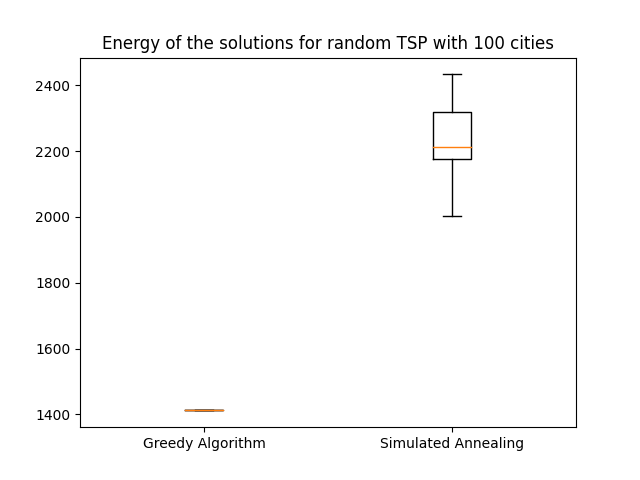
\includegraphics[width = \textwidth]{img/E100.png}
\end{subfigure}
\caption{\label{EBoth} Box-plot of energy for both algorithms on randomly generated TSP}
\end{figure}

On \autoref{E4N} we can see that as $N$ gets bigger the energies found by both algorithms are getting bigger as well. This is logical, since we have more cities to visit the path is longer.

\begin{figure}[H]
\centering
\begin{subfigure}{0.49\textwidth}
\centering
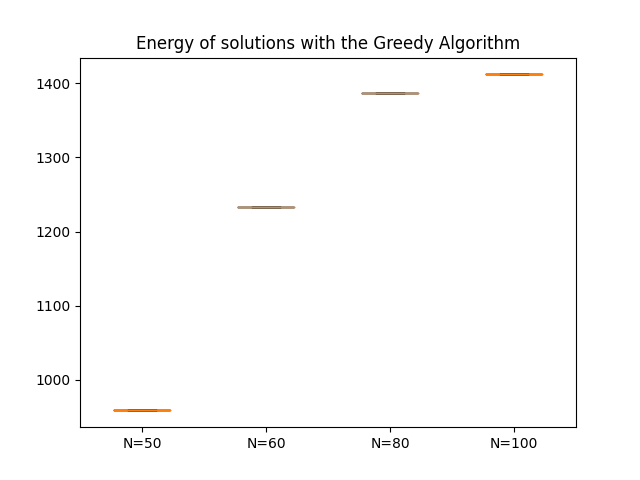
\includegraphics[width = \textwidth]{img/energyG.png}
\end{subfigure}
\begin{subfigure}{0.49\textwidth}
\centering
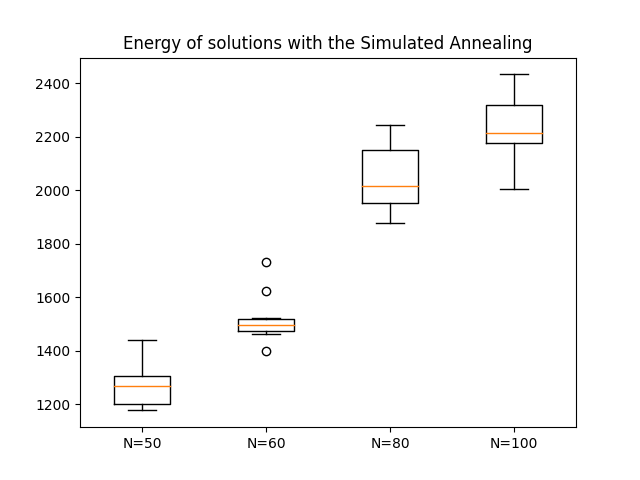
\includegraphics[width = \textwidth]{img/energySA.png}
\end{subfigure}
\caption{\label{E4N} Evolution of the energy for all four values of $N$. Left for the greedy algorithm and right for the simulated annealing.}
\end{figure}

Since the SA algorithm is probabilistic and since for a higher number of cities there is a higher number of possible paths, I thought that with a bigger number of execution there was more chances to find a better solution. To verify my hypothesis I tried to increase the number of time that I executed each algorithm on a same problem to see if it impacted the results of the SA algorithm. For TSP with 50 cities I ran the algorithms 50 times instead of 10 and this time the SA algorithm was some times able to find solutions with a smaller energy than the greedy one and in the other cases the best energies found were globally closer to the greedy one than before (just for one test there was no improvements but since increasing the number of time that we run the algorithm gives us more chances to find a better solution it does not mean that it will always be the case). I increased the number of executions to 100 and the results were even more closer and a better solution was found more often.\\
On \autoref{E50} we see on example of my tests, the energy found with the greedy algorithm is $1143.305564155386$ and the best energy found with SA is $1201.0235165104432$ when run 10 times, $1188.5519076724472$ when run 50 times and $1144.7440413689035$ when run 100 times.In this example the SA algorithm did not find a better solution than the greedy algorithm but the best energy when ran 100 times is really close and we can clearly see the improvement. We can also note that, in the same way that running more times the algorithm gives more chances of finding a better solution, when ran more times the worse result returned by the algorithm is higher. therefore the mean often does not improve.\\
I didn't continue to experiment by increasing more the number of time that the algorithms are run or by taking a higher value of $N$ because the computation time was just to long. But I am confident that the improvement in the solutions when increasing the number of times that we run the algorithm will work the same for higher $N$.

\begin{figure}[H]
\centering
\begin{subfigure}{0.32\textwidth}
\centering
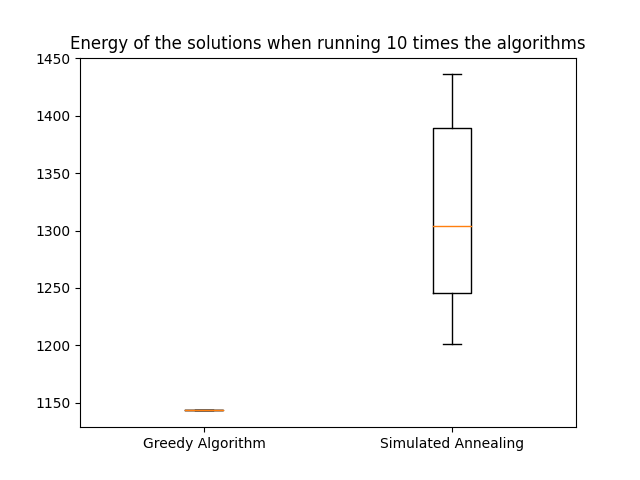
\includegraphics[width = \textwidth]{img/E50_10.png}
\end{subfigure}
\begin{subfigure}{0.32\textwidth}
\centering
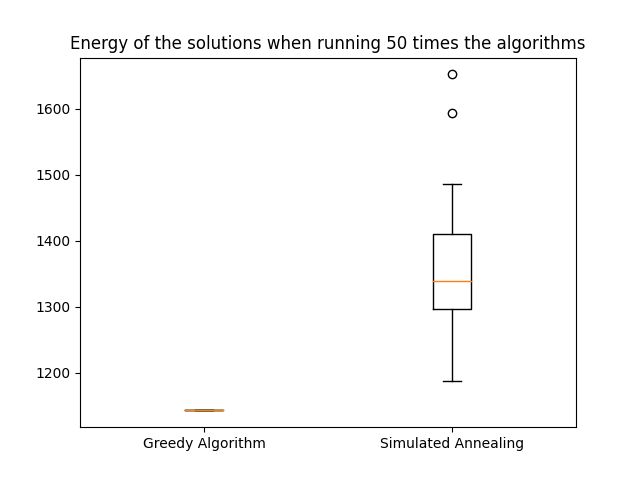
\includegraphics[width = \textwidth]{img/E50_50.png}
\end{subfigure}
\begin{subfigure}{0.32\textwidth}
\centering
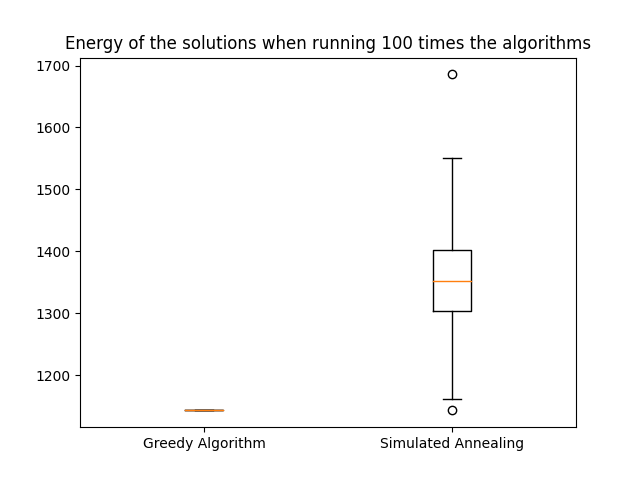
\includegraphics[width = \textwidth]{img/E50_100.png}
\end{subfigure}
\caption{\label{E50} Example of the energy obtained when running the algorithms 10, 50 and 100 times on a same problem.}
\end{figure}

\subsubsection{Computation time}

On \autoref{TBoth} we can see that for each size of $N$ the SA algorithm takes more time than the greedy algorithm. This was expected since we have a lot more iterations before returning a solution in the SA algorithm than with the greedy algorithm. We can also see that the more cities we have the more the difference between the time taken by SA and the time taken by the greedy algorithm gets bigger.

\begin{figure}[H]
\centering
\begin{subfigure}{0.49\textwidth}
\centering
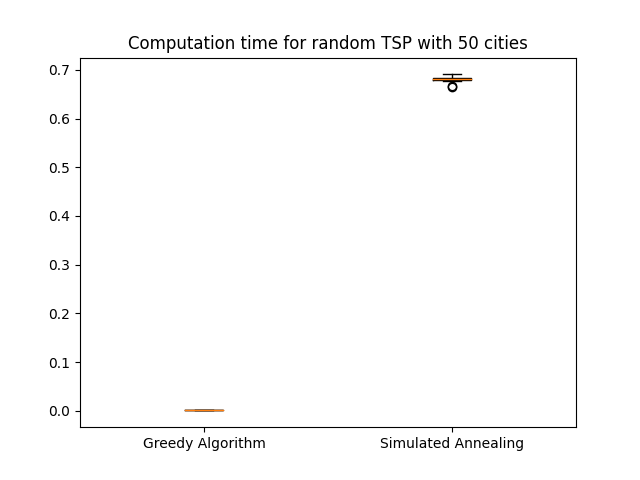
\includegraphics[width = \textwidth]{img/T50.png}
\end{subfigure}
\begin{subfigure}{0.49\textwidth}
\centering
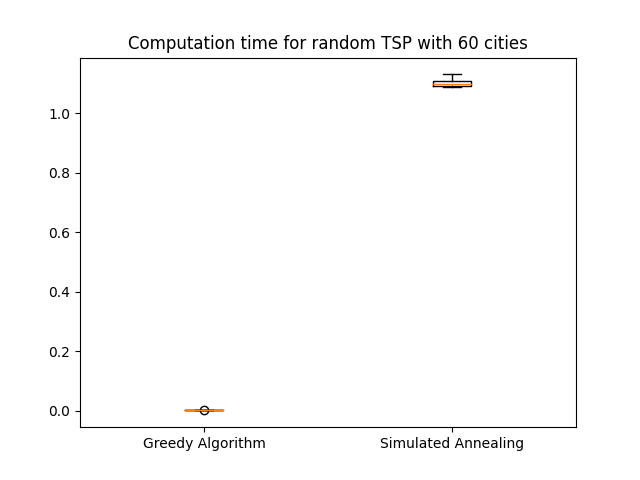
\includegraphics[width = \textwidth]{img/T60.png}
\end{subfigure}
\begin{subfigure}{0.49\textwidth}
\centering
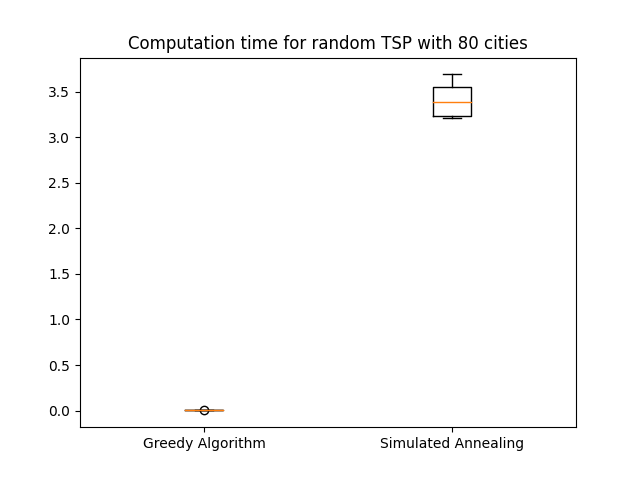
\includegraphics[width = \textwidth]{img/T80.png}
\end{subfigure}
\begin{subfigure}{0.49\textwidth}
\centering
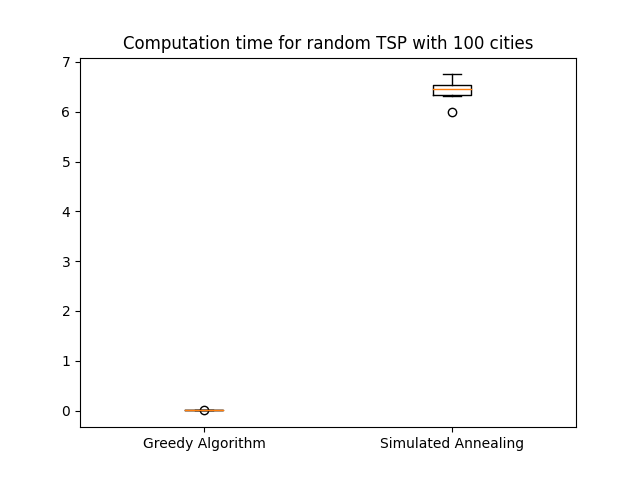
\includegraphics[width = \textwidth]{img/T100.png}
\end{subfigure}
\caption{\label{TBoth} Box-plot of computation time for both algorithms on randomly generated TSP}
\end{figure}

When we plot computations times of both algorithms separately (like on \autoref{T4N}) this gets even clearer. The increase of computation time is much slower for the greedy algorithm. This confirms that the time complexity of the simulated annealing is higher than the time complexity of the greedy algorithm.

\begin{figure}[H]
\centering
\begin{subfigure}{0.49\textwidth}
\centering
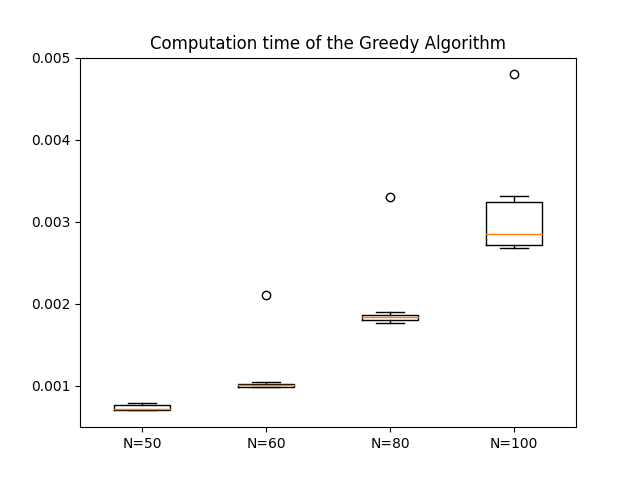
\includegraphics[width = \textwidth]{img/timeG.png}
\end{subfigure}
\begin{subfigure}{0.49\textwidth}
\centering
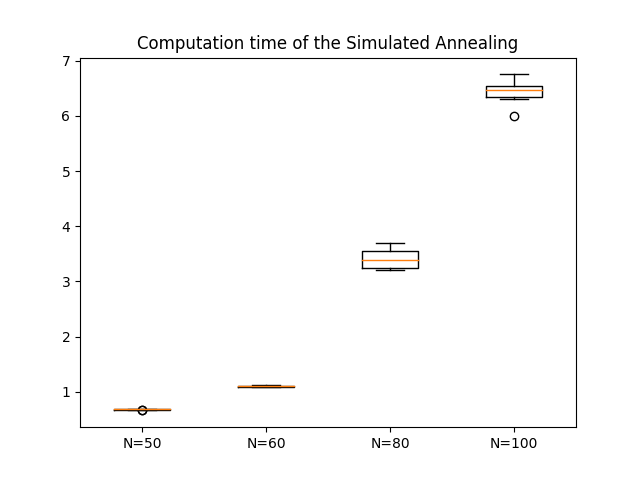
\includegraphics[width = \textwidth]{img/timeSA.png}
\end{subfigure}
\caption{\label{T4N} Evolution of the computation time for all four values of $N$. Left for the greedy algorithm and right for the simulated annealing.}
\end{figure}

\subsubsection{Conclusion}
From the results obtained on both experiment (tasks from a file and random TSP) we can conclude that, first, looking at the mean of the results for the simulated annealing is not very interesting since most of the time it is much higher than the best value found. Second, the simulated annealing algorithm does not always give better results than the greedy algorithm. However, if we can afford to spend more time computing the results, running several times the SA algorithm on a same TSP can provide a better solution than the greedy one (if the greedy solution is not the optimal solution).
\end{document}